\chapter{Approach}
\label{cha:Approach}
In the last section a few approaches have been outlined and discussed, that have successfully implemented methods regarding the creation of audios/music with a neural network approach. As seen, these have been mainly categorized in neural audio synthesis and neural audio style transfer. This work is mainly influenced from the area of neural audio synthesis, and can be categorized as such, as the methodology and workflow is strongly related to those works. Nevertheless regarding certain components, it has also its influence from the style transfer methods, despite not defining a specific content or style audio respective loss functions.\\

This chapter will therefore dive into the methodology and exact workflow of this works' solution, to the problem that also will help to derive the answers to the defined research questions. First an Overview/Motivation should provide the reader with the intended idea and an overview of the applied methods, to get a general understanding of the idea (see section \ref{sec:app_motivation}. Later on the single steps and components that are needed, to reach the desired functionalities, are getting in detail, starting with the pre processing. Further on the ML-Model (neural network) will get described, as well as the step that is done to synthesize new sounds. Further on, the required steps for (re)generating a listenable audio as well as an description of the used dataset for training and also all experiments conducted later on (see chapter \ref{cha:Experiment}).

\section{Motivation}
\label{sec:app_motivation}
Like mentioned in the beginning of this thesis, this work aims to explore the possibilities of machine learning techniques such as neural networks, to apply in the audio domain for sound generation. This idea is mainly inspired by the idea of taking two distinct audio sources and mixing their characteristics in order to generate a new sound. As seen in the previous chapter, this idea is strongly related to the image domain, where the "synthesis" of a new pictures based on two source images, is commonly known as image style transfer (point \ref{sec:rw_imgstyletransfer}). This technique, having a content image to be stylised with a certain style from another image, would mean for the application in the audio, to have a style sound to be transferred onto a content or target sound. Such methods are specifically known as audio style transfer and can either be applied to single notes or also whole audio samples or songs. Having the principle of content and style this would mean, that of one sound the global structure and rhythmical components get preserved while imposing style (e.g. the timbre) on it to generate audios. The details to these approaches, have already been outlined in the previous chapter, when describing some existing work around this topic.\\

Neural audio synthesis is another method for neural sound generation, which does not apply the principles of style and content audio. In the previous chapter, some insights could be gained, how neural audio synthesis can look like, as well as how it can be achieved using different methods and neural networks. Most of those methods, were showing promising results, either concerning the auditory quality but also the possibilities that arise in experimenting and designing sounds. Those methods were applying most of the time so called autoencoder networks, that can be used for dimensionality reduction of input data, as they have a so called "bottleneck" in the middle. \cite{hinton2006autoencoder} Because of this structure, the compressed data in this "bottleneck", can be seen as a representation for essential features that either can be combined/interpolated or directly synthesized. To generate synthesized audio, the solutions described in section \ref{sec:rw_neural_audio_synthesis} took advantage of the "decompressing part" of the network to generate in order audio data. The exact workflow and methodologies for sound creation, have already been mentioned in the chapter related works (see chapter \ref{cha:related_works}, point \ref{sec:rw_neural_audio_synthesis}).

Out of those methodologies, when having the idea of using two instruments' characteristics, to generate audio, the approach of \textit{Engel et al.} \cite{Engel2017} using convolutional and WaveNet-style autoencoders yielded the most promising and interesting results. This can be said especially in terms of output quality but also concerning its implementation and reproducability. With a provided interactive web application, the results of this solutions can be explored, whereas different sounds can be mixed based with a certain ratio. The results in the web application are based on the WaveNet-style autoencoder but according to the scientific article, the convolutional (baseline) yet also provides strong results. Implementing an approach with a WaveNet-style network would also go beyond the scope, not at least as the computational costs would be too high. As also some audio style transfer methods, especially the approach by \textit{Ramani et al.} \cite{Ramani2018}, are using convolutional autoencoders, this kind of network was chosen to be preferable, to be applied in this work. How (convolutional) neural networks work, especially concerning autoencoders, will get described later on. This gets done with special respect, on how those functionalities help to carry out neural audio synthesis, but also to gain general knowledge and a better understanding.

\section{Overview}
\label{sec:app_overview}
Based on the motivation and existing approaches, this work aims to propose a system, that uses a convolutional autoencoder network, for the task of neural audio synthesis. This systems' goal is to take two distinct audio samples as input, whereas the significant features, of those get extracted and interpolated, to (re)generate a novel sound in the end. In figure \ref{fig:toolchain} the general workflow of the toolchain is depicted in order to get an understanding, how this system is built up. 

 \begin{figure}[htb!]
	\caption{Overview of the proposed solution}
	\label{fig:toolchain}
	\centering
	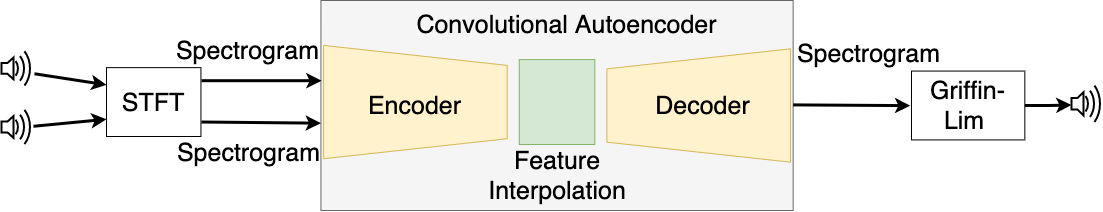
\includegraphics[width=\textwidth]{images/approach/Toolchain.png}
\end{figure}

Starting on the very left, two audios are taken and have to be brought into a suitable representation for this type of network. As audio is in its raw form a time-continuous signal and the input for convolutional networks are of a different shape (e.g. images) some pre-processing has to be done. In this case the short-term Fourier transform (STFT) is applied in order to generate a spectrogram, that shows the frequency spectra over the time. The frequency spectra contains on the one hand the magnitude (power) of the frequencies but also the phase information. For this purpose, only the magnitude data gets used, as recent publications stated that it contains the most descriptive data of an audio (spectrogram). The autoencoder model then takes the magnitude data as input, from which a compressed representation with the essential features gets generated by the lefthand (encoder) side. Having those features of two different audio samples, those get linearly interpolated, to generate one feature vector representing the "mixed" features of two instruments. This new vector, gets passed through the righthand (decoder) side of the network, which regenerates again spectral magnitude data of the same dimension as the input. In order to obtain a "playable" audio sound, it gets transformed back into time-domain with the Griffin-Lim algorithm \cite{Griffin1984} or the inverse short-term Fourier transform (ISTFT). The latter will be applied if there was no interpolation in the embedded space, as the phase information can be reused. Corresponding terminologies as well as a detailed insight into each step and its functionalities are given down below in the following points.

\section{Pre-processing}
\label{sec:app_pre-processing}
Pre-processing is the task of preparing raw data for a specific purpose. Moreover it is an important component of machine learning techniques, with respect to training neural networks. Deciding which pre-processing technique(s) to use on the one hand depends heavily on the type of ML-problem that has to be solved or even the training method that is chosen, but of course also on the type of data itself. As written before, for this work a neural network consisting of convolutional layers, has been chosen to be applied to the problem of neural audio synthesis. As convolutional neural networks are known for image processing tasks, they also can be applied for audio data, which has already been outlined in recent works in this field (see chapter \ref{cha:related_works}). In contrast to image data which most of the time has a 3D shape (width x length x RGB-colors), raw audio has a different structure in its data representation, as it is a time-continuous signal (1D-shape). To in order bring the audio data in a similar shape, it has to undergo some pre-processing steps. Some representations of audio that have a image-like shape and that got proven beneficial regarding neural audio synthesis, include e.g. log-magnitude spectrograms or Mel-spectrograms but also chromagrams and Constant-Q Transform as stated by \cite{choi2018tutorial}. Taking recent works into account, this work chooses to use the first representation as this one also got used more frequently and had promising results. As for comparison in the experimental part of this work, also the use of Mel-spectrograms will get assessed and discussed concerning the synthesis task and the performance of the neural network. 

As the practical part of the project to this thesis is implemented in python, a special library was used for the pre-processing part. For this part the library librosa \cite{brian_mcfee_2022_6097378} was used, as it provides practical functions for audio processing, that were considered as useful for this work. Special to mention here are the functionalities as calculating spectrograms (STFT) but also transforming spectral data back into time domain to generate playable audio data (ISTFT, Griffin-Lim).


\subsection{Spectrograms and STFT}
Spectrograms represent a 2D-representation of an time-continuous signal, which essentially shows the presence of certain frequency bands over time. Like previously said, there exist different forms of spectrograms e.G. log-magnitude and log-mel spectrograms. Especially speaking of the log-magnitude spectrogram whose calculation is based on the short-time Fourier transform (STFT) and thus on the Fourier transform. The Fourier transform, takes a frame of $N$ values of an (audio) signal and transforms it from the time domain into the frequency domain. Generally said, that the bigger the frame, the better is the frequency resolution. What this means in terms of calculating the spectrogram, will get outlined shortly. Whats also important to mention at this point is, that the result of the Fourier transform, consists of an array of $N$ complex numbers, which are mirrored in the middle. Every complex number in this array stands for a so called frequency bin in the signal. The real part of these numbers would represent the power/magnitude of this "bin" and the imaginary part gives information about the phase. Coming back to the frequency resolution, this for example means that when taking a one-second signal with a sampling rate $SR$ and performing the Fourier transform with length $N=SR$ on it, this would yield an array of $N$ values. The first value in the result depicts the signal's offset whereas all values from 1 to N/2 are the frequency bins with a resolution of 1Hz per bin. This means that each of this bin shows the magnitude and also phase of each frequency from 1 to N/2 Hz. The ongoing values in the result, show the same values except they are mirrored, as they depict the negative frequencies. Because of this behaviour, the second part can be omitted for further use. Now these values just show the frequency spectra of one time frame and do not incorporate more information about the change. To overcome this shortcomming, the Fourier transform can get applied to a series of frames of the signal in order to obtain multiple frequency spectras over time that get depicted as a spectrogram.\\

The calculation of multiple frequency spectras over time is done via the so called short-time Fourier transform. This form of calculation is widely used for pre-processing of audio data for ML-Tasks (for example see chapter \ref{cha:related_works}). When applying this transform, a few parameters have to be considered, as those influence the result but also the quality for the later workflow. One of the the most important parameters is \texttt{n\_fft} as it specifies the actual length of the signal-frame, on which the FFT (fast Fourier transform) gets applied to. This parameter therefore influences the frequency- but also time-resolution in the final spectrogram. To be mentioned regarding the official Librosa documentation, this should be a value of a power of two, as it speeds up the computation of the FFT behind. Another important parameter would be the \texttt{hop\_length}, which defines how much audio values are between the beginning of the first and the following frame. This means that when defining this parameter to \texttt{n\_fft/2} this would yield in a 50\% overlap of the following frame. Modifying this parameter, would mean to either increase or decrease the overlap and also the amount of time columns in the result, as more overlapping frames occur. The overlap of the frames is also coherent with the chosen window function for the STFT. As every time when the FFT gets applied to a frame, this one gets multiplied with a so called "window". Multiplying a signal frame with a window has to be done, as the FFT assumes, that the transformed signal is periodic (repeating itself infinitely). \cite{heinzel2002spectrum} This gets problematic when the input signal does contain frequencies that may not directly fall into a frequency bin, due to the FFT's frequency resolution. Due to the assumed cyclic continuation the Fourier transform will 'think' that there is a discontinuity and will spread therefore the power over all the spectrum. There exist multiple window functions such as "Hann", "Hamming", "Blackman", etc. which start at (almost) zero, rises to a maximum in the middle but falls again to (almost) zero at the end (symmetric). Multiplying the signal frame with such a window function helps to overcome this issue as it removes the discontinuity. On which window to chose, depends on the use-case of the application, whereas throughout this work a "Hann"-window was chosen all the time. Coming back to the relation with the window overlap, if no overlap would be used a lot of information of the signal would get lost. This is because when multiplying the signal frames with the window functions, this would bring very little or zero values at the beginning and end of the frame. \cite{heinzel2002spectrum} When having overlapping frames this issue would get corrected. Important here is again the amount of overlap as this is dependent on the window and its wideness. Using the "Hann"-window a common value for the overlap would be 50\% which was also considered throughout this work. This value is also beneficial later on, when performing the inverse transformation, back into time domain, but more on that in section \ref{sec:app_post_processing}. Beside of these parameters some more exist, for example for specifying the padding of the signal whereas in this work a constant padding on both sides of the signal has been used, which is also the default setting. \\

Now having the knowledge of the STFT and its parameters, it can be applied onto a signal, to generate a spectrogram. For example by using an audio sample with a sample rate of 16 kHz and applying the STFT with a \texttt{n\_fft} value of 1024 and a \texttt{hop-length} of 512 this would result in a spectrogram with a frequency resolution of 15,625 Hz and time resolution of 64 ms. As explained before, the values of the result, consist of complex numbers which contain the magnitude but also the phase at each frequency bin. By setting this result absolute, or calling the function \texttt{librosa.magphase(spectrogramm)} the real magnitude data can be obtained, whereas the latter also retrieves phase information in a separate vector. The magnitude here displays the energy values of the spectrogram, whereas for further processing and also to be better displayable those get converted into a dB-scale. \footnote{normally the magnitude would need to get squared to obtain the power, but in this case magnitude without squaring was taken} This function also takes a reference value that gets set to 0 dB, which in this case will be the maximum value of the magnitude spectrum. As for post-processing when converting the dB-scaled data back into energy, also a reference value is needed, this one gets preserved, in order to get the same scaling as in the original input. Finally when having the log-mag spectrograms in dB, those were considered for the training of the neural network afterwards. An example of a log-mag spectrogram can be seen in figure \ref{fig:spectrogram}. As also the phase information was obtained when calculating the magnitude data, this one was also preserved next to the energy reference value for the recreation of signals, as it is needed there (this will mainly affect the recreation of single samples, without interpolation in embedded space, but more on that later on).


 \begin{figure}[htb!]
	\caption{STFT log-mag spectrogram of a guitar note}
	\label{fig:spectrogram}
	\centering
	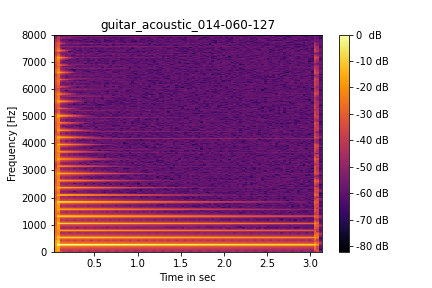
\includegraphics[width=0.8\textwidth]{images/approach/guitar_acoustic_014-060-127.png}
\end{figure}

This section describes the general workflow of the pre-processing from taking a signal and converting it into a spectral representation. This workflow is a basis on which different experiments with different parameterization (size of n\_fft, etc. ) of the calculation of the spectrograms but also with additional steps (log-mel scale, additional framing, etc.) are being made. Those steps will get mentioned later on in chapter \ref{cha:Experiment} when describing the experimental part of the thesis.

\section{ML-Model}
\label{sec:app_model}
The main or core component of every machine learning project is of course the model itself, as it achieves the main task of prediction or inference to a given problem. Those models exist as different technologies that perform regression tasks or even classification tasks. Dependent on the use-case, but also the kind of data that is present, different models are better suited or not. To count technologies, there exist the KNN-Algorithm, Decision-Trees, Random Forests, Support-Vector-Machines (SVM) but also neural networks which can be applied in a variety of usecases. Especially the latter, the neural networks, are able to achieve a variety of different tasks, as they are highly adaptive regarding their topology, used layers, but also the size and shape. Those variety of different tasks spread across different domains, so also for images and audio. 

\subsection{Neural Networks - Introduction}
Generally said a neueral network can be seen as a graph of connected nodes  with numeric values that can achieve transformations between patterns using message-passing algorithms. \cite{Jordan1996neuralnets} Those nodes are commonly structured in layers, where there especially exist certain nodes or even layers that are seen as input nodes/layers and some as output nodes/layers. Between the input and the output there can also exist so called hidden layers, expanding the depth of the network. The links between the nodes, that get also called neurons, are connected via links, that are parameterized with weights, that get optimized using learning algorithms. Each neuron receives its weighted input (activities) of its connected predecessors, which get converted into a single output that gets broadcast to all its connected successors. \cite{hinton1992neural} The latter involves a so called input-output function which is also commonly known as activation function (e.G. ReLU, Sigmoid, Softmax ...). Important to know, is that the weights on the connections define how much this value influences the input of the connected node. 
When a neural network gets trained to a specific problem (e.g. classifying certain images), using predetermined training data, the output of the neural network gets compared with the desired one, resulting in a certain error (metric). To minimize this error, the weights in the network get adapted by back-propagating the error through all the layers, to the beginning. On this way it changes the influence of certain connections and therefore the overall outcome. This procedure gets repeated on all training data over several iterations, until the error gets low to produce the desired output. The initialization of the network and its weights are often random, which also means that every training run starts and progressses differently.

Depending on the problem to solve / what's the desired output, neural networks can be trained using labeled data (supervised) but also just by minimizing a cost function (unsupervised).\cite{oshea2015introductionConv} More details on the learning will get mentioned later on when explaining the model itself. 

\subsection{Convolutional Neural Networks}
\label{subsec:app_conv}
In this approach, due to the promising usage in existing solutions, a convolutional neural network has been chosen as model. Convolutional neural networks are a type of networks, that get primarily used for tasks in the image-domain for example to recognize patterns in pictures or classification, but also like seen in chapter \ref{cha:related_works} for image style transfer. They have the advantage over traditional neural networks, that they can cope with the dimensionality of pictures (width x height x colors/depth). The layers containing convolutional nodes have as learnable parameters, so called kernels. \cite{oshea2015introductionConv} Those kernels, if taking a 2D-Convolutional layer, are normally small in width and height (e.g. 3x3) but span the whole depth (channels) of the input (in the case of RGB-pictures depth of three). Those kernels calculate the skalar-product for each value contained in the kernel and the input map. This yields, having e.g. a 3x3 kernel operating on a 3x3 field, in a single value. This value is the weighted sum of the kernel's values and from those of the input vector. This operation will be applied to each 3x3 field along the spatial dimension of the input, resulting in a smaller activation map. One can also apply padding around the input, to preserve the dimensionality. Furthermore a stride can be defined, which defines how much these convoluted fields overlap, as using a bigger stride would result in a smaller overlap. Having also a smaller overlap would result in a much smaller activation map. 
For example taking a 7x7 input, by applying a 3x3 kernel with no strides and also no padding, this would yield an output field of 5x5. With a padding of 1x1 the output would be of the same size. Finally if the stride would be 2, the output field would be of 3x3.
Through training of the network and back-propagating the error, those values in the kernel get adapted in order to learn certain/important features or patterns on which a classification or pattern recognition can be made (easier). As it got here described for 2D-convolutions, depending on the input dimensionality it can be also be applied as 1D-convolutions or even 3D-convolution. 


With the knowledge, that such convolutions are successful on image data, those can be also applied on audio provided in the shape of a spectrogram. As described in the previous section (see \ref{sec:app_pre-processing}) spectrograms can be described in a "picture-like" shape having the dimensions of frequency x time with a depth of one. Speaking of that, the spectrogram can be seen as a grey-scale image. The energy in different frequency bands over time with its variations, can be seen as "recognizable" patterns. 
Taking a 2D-convolution, the kernel (e.g. 3x3) takes a 3x3 frame of frequency x time which results in one value. Summed up, this results in an activation map smaller or equal (if zero padding is used) than the input. After training on different samples and iterating several times, those activation map would contain the most significant features or characteristics of the spectrogram for example when training on classification.
Depending on the chosen hyper parameter for the amount of output channels (depth), the resulting activation map can be of depth one or even deeper. 

As mentioned before, each neuron in a neural network has an activation function, which is also the case for convolutional neural networks. As there exist different kinds of activation functions, for this approach mostly ReLU (Rectified Linenar Unit) activation functions got used but also LeakyReLU. Additional to this activation function, BatchNormalization gets applied after each convolutional and ReLU non-linearity component. The choice is mainly based on already existing approaches like from \textit{Ramani et al.}\cite{Ramani2018} and \textit{Engel et al.}\cite{Engel2017}, as it was proven to yield promising results in combination. According to \textit{Ioffe ad Szegedy} \cite{ioffe2015batch} applying Batch Normalization also improves the training speed (number of iterations/epochs) and enables use much higher learning rates. Furthermore it acts a regularizer, so that overfitting-reducing technologies, such as Dropout, can be omitted.

\subsection{Autoencoder}
Neural networks exist in different shapes and compositions, depending on desired work it should fulfill. Whereas some networks e.g. for classification of a given input, might reduce the width of the layers towards the end, some are designed to have a so called "bottle neck". This means, that this kind of network, contains a smaller central layer then the input, but at the end again a bigger layer (eventually same size of input layer). \cite{hinton2006autoencoder} Those networks are called autoencoder, in which the first part of the network (until the smaller central layer) gets called "encoder". The second part beginning at the small central layer, that is getting bigger towards the end, gets called "decoder". These parts are called this way, as for the encoder part, it "encodes" the high-dimensional input data to a low-dimensional representation (output of small central layer). The counterpart is therefore called "decoder" as it decodes the low-dimensional data, to bring it again to a higher-dimensional representation (mostly same as input). The lower dimensional output of the small central layer, can be named differently, as for example "code", what \textit{Hinton et al.} does when describing the work of autoencoders in his publication \cite{hinton2006autoencoder}. Some other common names would be e.g. latent space, embedding space, encoding or embedded data. This principle of dimensionality reduction, therefore means, that the encoder part extracts the most important or characteristic data, from which the decoder is able to reconstruct the input data.

In the related works chapter (\ref{cha:related_works}) a few works have made use of this principle to extract "characteristic" features for audio data and synthesize audio from it, by altering them. This knowledge encouraged this work to also make use of this principle to synthesize audio by using autoencoders. Especially when having the extracted audio features as encodings, those can be modified (easier), to in order synthesize novel sounds from them using the decoder part of the network. 
Combined with the knowledge to apply convolutional networks to audio spectrograms and the advantages of autoencoers to extract features from the input, the model in this work is designed as convolutional autoencoder. Also the works of \textit{Ramani et al.} or \textit{Engel et al.} made use of these kind of network to generate novel sounds. Figure \ref{fig:app_autoencoder} shows the basic autoencoder network structure which is used throughout this thesis work. To be mentioned, the whole implementation of the neural network for this work has been achieved with the deep learning library PyTorch.\cite{paszke2019pytorch}

\begin{figure}[htb!]
	\caption{Basic autoencoder structure used throughout this thesis}
	\label{fig:app_autoencoder}
	\centering
	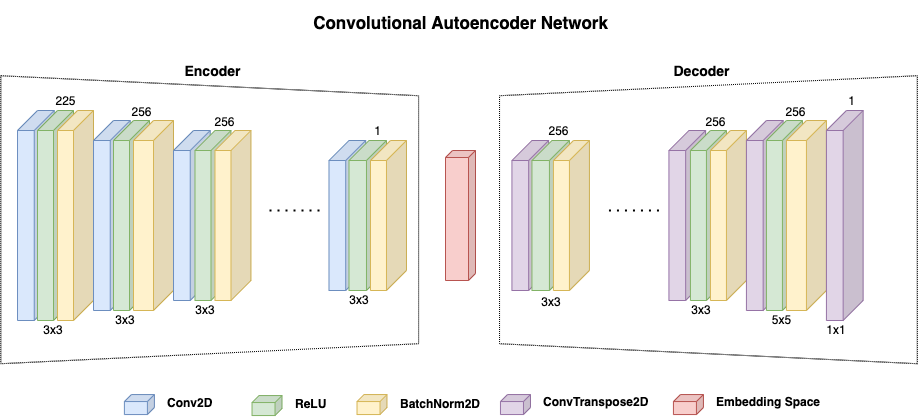
\includegraphics[width=\textwidth]{images/approach/autoencoder.png}
\end{figure}

In this figure, the depicted autoencoder, gives an insight of which components and layers it is composed. The amount of layers as well as the parameters shown in this sketch, are just an example, as throughout the experimental part, those get varied. Therefore, the dotted lines in this figure, act as a placeholder for possible more layers on each side in the network. The numbers above the individual layers, represent the amount of output channels (depth) and those on the bottom, represent the kernel size. Some paragraphs before, it has been mentioned, that in this approach the convolutional layer gets equipped with ReLU activation function and BatchNormalization. This also gets visualized in this figure, where each layer is shown as combination of sub-layers that incorporate those three components. Speaking of the composition of the layers, it can be seen in the decoder part, that instead of a convolutional layer, a convolutional transpose layer is used. That is because of the nature of convolutions, as their output is always smaller or equal sized, which has been mentioned under point \ref{subsec:app_conv}. As the decoder part generates output that is bigger than its input, the layers have to perform upsampling. In convolutional nets this is typically done via the convolutional transpose layer.\\

This transposed convolution is not the reverse operation of a convolution, but it is more a operation to recover the shape from the convolutions input. \cite{dumoulin2018guideconv} Taking the convolution example from above, by taking as input a 5x5 field and applying the transposed convolution, with a kernel of 3x3 this would result in a field in 7x7. The equivalent of this operation would be a convolution with the same kernel, on an input of 5x5, with 2x2 padding (padded input = 9x9), as this would result in a 7x7 output too.
When in the convolution, striding was applied, this also works for the transposed convolution. Again when having the 3x3 input, by applying a 3x3 kernel with a stride of 2, this again results in a 7x7 output field. To be mentioned, the striding parameter for the transposed convolutions, defines how much zeros are added between the values of the input. This means, when taking the previous example, that the 3x3 input gets one column respective one row of zeros inserted after each value to result in a 5x5 field.

With this knowledge, convolutional transpose layers are best suited to be in the decoder part of convolutional autoencoder networks. Coming back to the architecture of the convolutional autoencoder in figure \ref{fig:app_autoencoder}, those convolutional transpose sublayers are also coupled with ReLU activations and BatchNormalization, with an exception to the last layer.\\

Having this kind of autoencoder for this approach and the idea to extract features of spectrograms using convolutions, this models task is to encode and decode spectral audio data. The network is therefore configured, to produce an output of the same dimensionality as the input of the encoder. Like mentioned above, the output should be a reconstruction of the input, that gets inferred, by decoding the extracted features in the embedded space. To achieve this goal of reconstructing the input, the network has to be trained, through minimizing a specific error. In some cases also maximization is desired, but is dependent on the error score and the desired outcome. In the case of an autoencoder, this works by comparing the output of the decoder with the input of the encoder, by calculating the difference. Generally said, depending on the outcome and the goal of a training, there exist different metrics like mean squared error (MSE), root mean squared error (RMSE), mean absolute error (MAE) but also more specific formulas. Throughout the literature, those error or error functions are also often called cost (functions) or loss (functions). For the experimental part of this work, the choice has been made, to use MSE as error metric, as it has been used successfully by some existing works. 

To minimize this error an optimization of the network has to be made, which will be done through back-propagating the error score. Through this step, the parameters (weights, bias, convolutional kernels, etc.) get adapted according the error, which in the best case, improves the score and thus the output of the network. In this work the output of the network are reconstructions of spectral data for example slices of spectrogram. As having the encoder-decoder structure, those output data get reconstructed through the decoder, which takes the encoder output as input. As mentioned before, this generated data of the encoder, is a compressed vector, consisting of the most significant extracted from the input. Depending on the configuration of the network, especially the encoder part, this vector also called encoding, can be of different size. This is because, when using more convolutional layers with strides, the output of each layer gets more downsampled, which results in a smaller encoding. As a consequence, the decoder part has to learn to regenerate spectral data from this encoded vector. This vector therefore is a compressed representation of the models input, which contains the most significant characteristics, of this specific spectrogram and further on, of the sound. All in all regarding the learning, it can be said, that the encoder learns to extract essential features, from which the decoder learns to regenerate in the best way, the input.

Altering those encodings, has therefore the consequence, that the output of the decoder is different, and thus will be a novel, synthesized sound. More on how it should get altered, gets discussed later on.
Choosing the right compression, is also an important part, that influences the outcome and thus the quality of the desired model output. Too much compression, may lead to the fact, that the decoder has too less information to infer the desired spectral output, which in order results in poorer quality of the resulting audio. On the other hand having, less compression, results in embeddings being not significantly smaller then the input, containing less important data too (e.g. noise). It also may gets more difficult to alter those encoded vectors. Throughout this work, different amounts of compression have been applied in the experimental part, which get discussed later, including the impacts and observations made on that. Knowing those properties and behaviour of the autoencoder model, this strengthens the idea, to apply autoencoders for the use of neural audio synthesis.\\


\subsection{Optimizer}
Coming back to the training process, where the network gets optimized, in order to minimize a certain error function and as consequence helps the network to converge. For this optimization, different strategies exist, where hyper-parameters such as learning-rate or weight-decay play an essential role. Those optimizations are on a large scale, stochastic gradient-based techniques, to which algorithms such as stochastic gradient descent (SGD) or Adam can be counted. Those algorithms influence and improve the convergence which means to find a minimal error. Throughout this implementation the Adam optimizer \cite{Kingma2014} has been chosen, as it is used widely in recent publications where promising results, could be achieved. Also regarding the training process in this work, Adam optimizer was proven to be advantageous, in contrast to SGD. The parameters that have been found to have the most impact on the optimization process during training, are the previous mentioned learning-rate and weight-decay. To be mentioned, the learning-rate specifies how "fast" the model actually learns while weight-decay works as a penalty for the weights optimization to prevent overfitting. If the learning rate is chosen rather big, then the network learns faster, but because of its big steps or jumps, it could miss out the optimal solution in the solution space. Also it could happen, that when optimum is found, that it "jumps" out again. In this case a smaller learning rate would be desirable, as it makes smaller steps. Choosing it too low, would end up in a slow training where also large areas of the solution space are not visited. The latter leads to get stuck in a local minimum. Therefore it is important to choose the right size of learning rate, but this issue depends also on the problem size and type of network. In this work different learning rates have been applied throughout the experimental part where also different findings could be made, but this will be shown and discussed later on in this thesis.\\
With this knowledge, it can be stated, that a high learning rate, could be advantageous at the beginning of the training process, in order to rather find a global optimum and explore the solution space. In order to prevent, to jump out of minimum, a smaller learning rate would be desirable later on in the training. For this case, there exist some mechanisms to decrease the learning rate, later on in the training, especially when detecting "oscillating" due to a too large learning rate.\\
In this works' implementation, for the start of the training a specific starting learning rate has been set, while throughout the training, it gets adapted, when no more optimization and eventual oscillation gets detected. 


\section{Synthesis of novel sounds}
\label{sec:app_interpolation}
Having now covered, the important properties of the pre-processing but also of the applied machine learning model, this section explains the methodology to synthesize a novel sounds. In the chapter \ref{cha:related_works} where related works got discussed, an insight could be gained, on how different works tried to synthesize audio with their neural networks. For example \textit{Colonel et al.}\cite{colonel2017improving, colonel2018autoencoding, Colonel2020} suggested in their works, to synthesize novel sounds, through directly activating the innermost layer. This means after training, for the sound creation process, the encoder part gets omitted. For example in the case where they had a network with 8 neurons at the encoders bottleneck, 8 different values could get defined, within a certain range. The decoder part then created, based on its training on recreating spectrograms, spectral data that got converted back to time domain to form a synthesized playable sound. 

\subsection{Interpolation in latent space}
Having this as one possibility, to use in particular autoencoders as tool for audio synthesis, there also exist some more interesting approaches. One of those got applied by \textit{Engel et al.} \cite{Engel2017} but also \textit{Roche et al.} \cite{roche2019autoencoders} where they also made use of the latent space encodings. Contrary to omitting the encoder part, those works aimed to utilize the whole network, as no direct activation of the innermost layer is considered. Instead the authors proposed to take the encoded values of two different audio samples (possibly two distinct instrument) and combine them via linear interpolation. The interpolation process in order yields a vector of interpolated values. This new vector, can be seen as a modified encoding, which gets processed by the decoder part, resulting in spectrogram-like vector. The result of this process is then a synthesized spectrogram, that aims to contain features of the two input sounds.

As the latter methodology corresponds the most with the initial idea, to synthesize audio based on the characteristics of two instruments (e.g. guitar and synthesizer), this method was chosen to be implemented to carry out experiments on the creation of novel sounds.

To explain this method in more detail, the encoded vectors of two audio samples serve as basis. Then each of this vector is taken, to interpolate a value that lies on a linear line between the value at a given index in one vector with the corresponding value of the same index in the second vector. To mention at this point, those vectors are of the same length. The result then is a new array containing the interpolated values of those two vectors. This procedure gets repeated for each encoded output of one sample with the corresponding output of the second sample. Knowing the fact, that those encoded values represent the most significant features and probably the characteristics of the note, the result can be seen as a combination of those characteristics. Decoding those, will then end up in having a spectrogram, containing the characteristics of both instruments. How this procedure and its results look like, with the actual experiments, gets shown later on in this work. 

\section{Post Processing}
\label{sec:app_post_processing}
It has been discussed, that regarding neural audio synthesis, the audio data can appear in different shapes. As there exist approaches, that focus on time-domain signal like the WaveNet-style autoencoder from \textit{Engel et al.}, there also exist those who operate on spectrograms using convolutional networks. As mentioned before, this work emphasizes on the use of a convolutional autoencoder, that takes spectrograms or spectral data as input. In the case of this autoencoder, the output is of the same shape as the input and therefore also a spectrogram. To generate again a playabele or listenable audio, this one has to get converted back into time domain. There exist many different methods, to achieve this, while this also depends heavily on the data that is present. As stated in section \ref{sec:app_pre-processing}, when spectrograms are calculated via the STFT, the output vectors are complex valued. To be mentioned, that without modification or further utilization, via the inverse STFT (ISTFT), this result vector can get converted back into time domain without loss. For achieving this task, it is necessary that the magnitude but also the phase information has to be present, combined in a complex number. As this autoencoder just operates on the magnitude data of spectrograms, there is no phase information present in the output of the network. At this point, multiple ideas can be applied, depending of what is done throughout the process. This means, that when there is no modification in latent space, i.e. value interpolation, the original phase information can be reused, to in order apply the ISTFT. As mentioned previously the phase information gets preserved for exactly this case. 

In the second case, where modification steps are performed, like here the interpolating of two sounds' embeddings, there is no phase information present, that can be used. To overcome this issue, there exist techniques that can approximate the phase information. One of those techniques, which is also probably one of the most prominent ones, is the Griffin-Lim \cite{Griffin1984} algorithm that tries to estimate the time-domain signal based on just the magnitude data. With this algorithm the phase gets randomly initialized, and with alternating forward- and inverse STFT, estimated. For the calculations of the audio signal, again the python library \textit{librosa} \cite{brian_mcfee_2022_6097378} has been used, as it provides the inverse STFT but also implements the Griffin-Lim algorithm. According to the documentation of \textit{librosa}, a so called "fast" Griffin-Lim algorithm is applied, which got developed by \textit{Perraudin et al.} \cite{Perraudin2013}. The difference here is, that this one utilizes a additional momentum parameter which helps to accelerate the convergence of the estimation. 

Some further note here, as when the pre-processing steps (see section \ref{sec:app_pre-processing} have been examined, that some certain parameters have to be taken care of. These are especially, the \texttt{n\_fft}, \texttt{hop\_length} but also the \texttt{window}. It has been mentioned, that e.g. the \texttt{hop\_length} was chosen to be half of the \texttt{n\_fft}, to ensure a 50\% overlap of the STFT frames. Furthermore the "Hann"-window was chosen, to be multiplied with the signal frames, to avoid discontinuities. Again, those also appear in the inverse STFT as well as Griffin-Lim. In order to obtain the best result, it is important, to apply the same values with those parameters. As the inverse Fourer transform gets applied to each vector in the spectrogram, this results in single time-domain frames that have the length of \texttt{n\_fft} (original length). With the knowledge of the window and the overlap, those single frames, get "overlap-added", which results again in the full length audio sample. 

Before applying the the inverse calculations on the auteoncoders output, it has to be considered, that the autoencoder works on the db-scaled magnitude. As a consequence the output therefore is also db-scaled. To apply the inverse calculations, the output gets back into energy. For this case a reference value, has been preserved from the pre-processing stage, to in order obtain the (almost) same scaling again in the output signal. For the experimental part some more steps also got applied, like scaling the energy according to the average energy present in the original spectrograms. This step should also correct and improve the resulting sounds. More on that in chapter Experiments (\ref{cha:Experiment}), but also later on when examining and discussing the results.\\


\section{Dataset}
\label{sec:app_dataset}
As machine-learning models including neural networks, have to get trained, in order to deliver accurate results, data is needed on which it should get trained on. To get compelling results, it is not only important to have an appropriate model configuration or pre-processing chain. The choice of an appropriate dataset therefore is also of high significance. As seen in related works, datasets can either be self-generated or taken from a public available data-source. As in the case of this work, the model operates on audio data, a dataset of musical notes is desirable. Generating sufficient data, on ones own, is a task that would take a significant amount of time. Not only as this dataset preferably should contain a large amount of audio samples, those also should be highly divers such as different instrument sources or different pitches. Not only is it an advantage for the training of the neural network to have lot of samples and diversity, as it helps to improve the learning process and generalization within the neural networks. Moreover it is also advantageous for this kind of work, as when having many different instrument sources and available notes, more interesting combinations with regard to audio synthesis can be made.

\subsection{NSynth Dataset}
Exactly for this kind of approach a big dataset consisting of musical notes called "NSynth", has been made publicly available by \textit{Engel et al.}. \cite{Engel2017} This dataset consists of a total of 306 043 musical notes that have a unique pitch, timbre but also envelope and has been created for the idea of neural audio synthesis. This amount of musical notes incorporate monophonic audio snippets, sampled at a rate of 16kHz, of 1006 different instruments. Every note is of a specific pitch, ranging over every note of a standard midi piano (21-108). This results in having 88 different pitched notes, in the best case, as not every instrument is capable of producing all different pitches. The average amount of pitches is therefore, according to the scientific publication, 65.4 per instrument. With more detail, each audio sample belongs to a certain instrument family which could for example a keyboard, guitar, organ, bass, brass and so on. Further on they can be distinguished of their source, being either produced acoustically, electronically or synthetically. All these specifications make this dataset, highly attractive for this kind of work, as well is it publicly available\footnote{\url{https://magenta.tensorflow.org/datasets/nsynth}} for free and already successfully used for neural audio synthesis. Regarding the use for machine learning tasks, on their website, they provide the dataset already, splited up into a training, validation and test set which do not overlap at all. To specify, the training set consists of 289 205, the validation set of 12 678 and the test set of 4 096 examples. For this purpose, it has been chosen, to take these splits as they are, for the training, validation and finally testing stage.